\documentclass[tikz,border=15pt]{standalone}
\usepackage[dvipsnames,svgnames,x11names,table]{xcolor}
\usepackage{tikz}
\usepackage{amsmath,amssymb}
\usetikzlibrary{shapes.geometric, arrows.meta, positioning, calc, fit, backgrounds, decorations.pathreplacing}

% =============================================================================
% COLOR DEFINITIONS - Mini-SepVAE
% =============================================================================
\definecolor{inputcolor}{RGB}{158, 158, 158}
\definecolor{encodercolor}{RGB}{76, 175, 80}
\definecolor{featurecolor}{RGB}{156, 39, 176}
\definecolor{commoncolor}{RGB}{255, 193, 7}
\definecolor{disease1color}{RGB}{244, 67, 54}
\definecolor{disease2color}{RGB}{33, 150, 243}
\definecolor{latentcolor}{RGB}{233, 30, 99}
\definecolor{routecolor}{RGB}{255, 152, 0}
\definecolor{decodercolor}{RGB}{0, 150, 136}
\definecolor{outputcolor}{RGB}{158, 158, 158}

\begin{document}
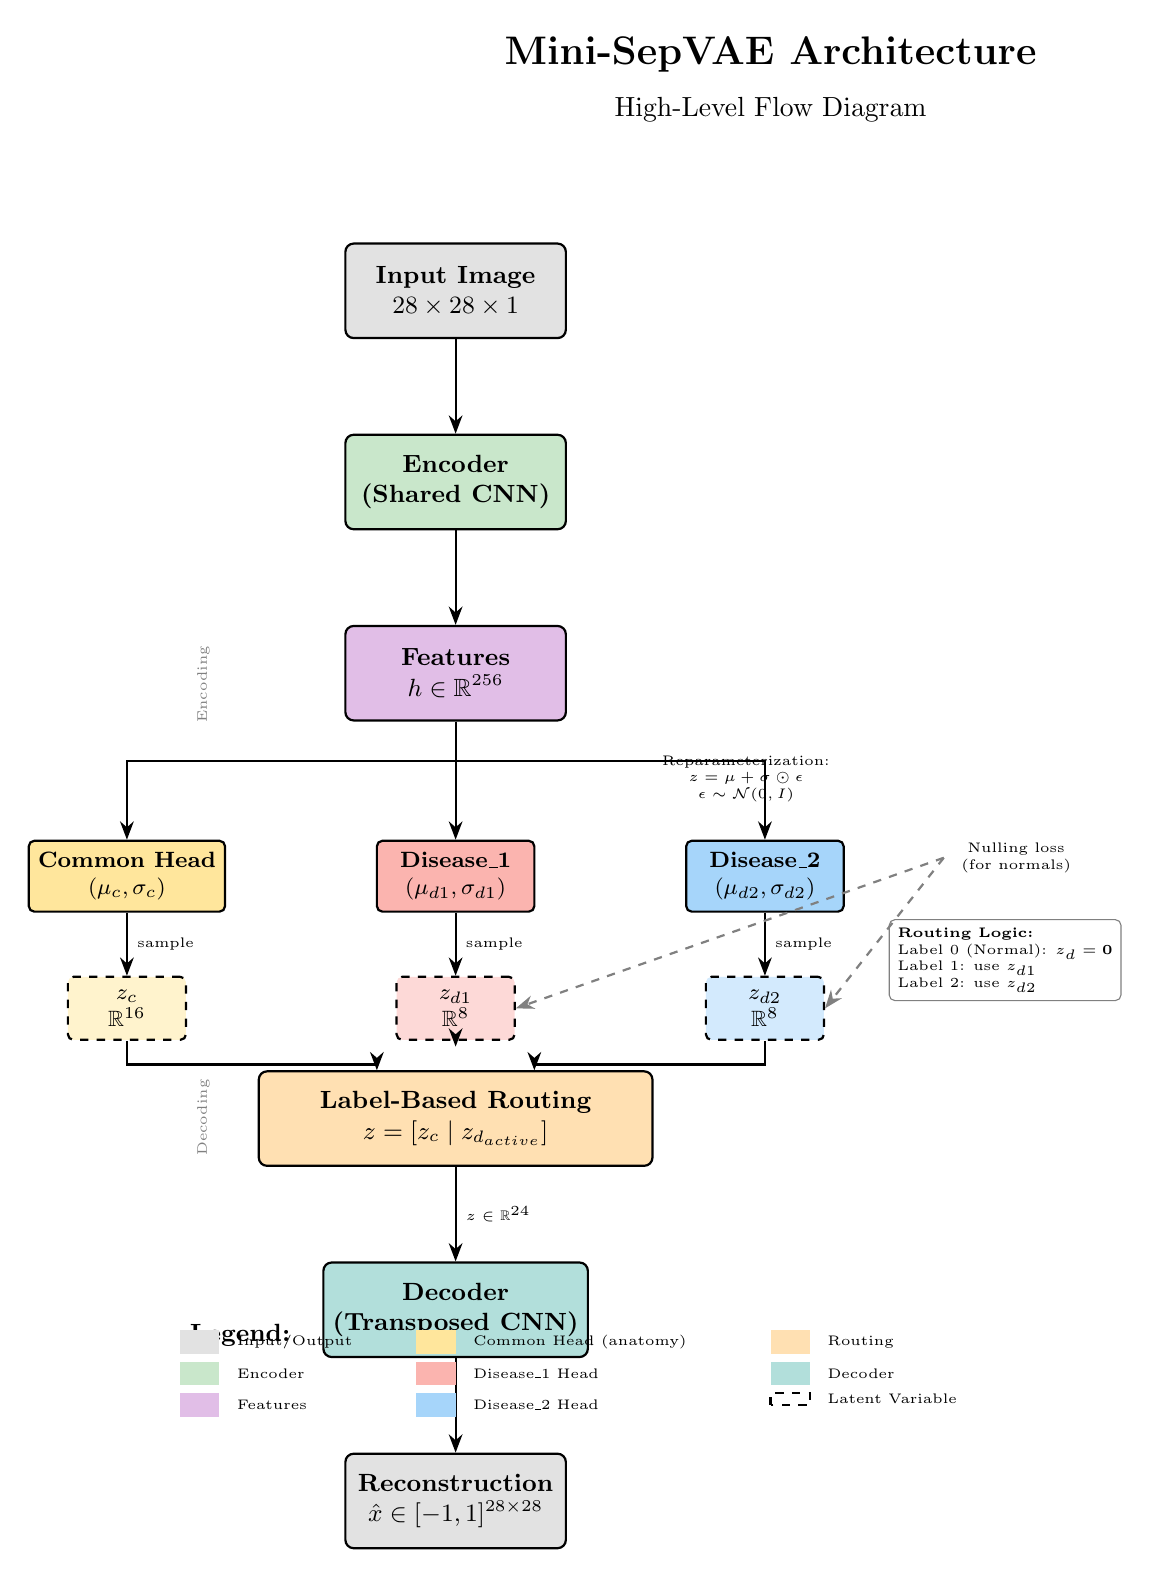
\begin{tikzpicture}[
    >=Stealth,
    node distance=1.5cm,
    block/.style={
        draw, thick, rounded corners=3pt,
        minimum width=2.8cm, minimum height=1.2cm,
        font=\small\bfseries, align=center
    },
    smallblock/.style={
        draw, thick, rounded corners=2pt,
        minimum width=2cm, minimum height=0.9cm,
        font=\footnotesize\bfseries, align=center
    },
    latentblock/.style={
        draw, thick, rounded corners=2pt, dashed,
        minimum width=1.5cm, minimum height=0.8cm,
        font=\footnotesize, align=center
    },
    arrow/.style={->, thick, >=Stealth},
    dasharrow/.style={->, thick, dashed, >=Stealth, gray}
]

% =============================================================================
% TITLE
% =============================================================================
\node[font=\Large\bfseries] at (4, 11) {Mini-SepVAE Architecture};
\node[font=\normalsize] at (4, 10.3) {High-Level Flow Diagram};

% =============================================================================
% INPUT
% =============================================================================
\node[block, fill=inputcolor!30] (input) at (0, 8) {Input Image\\$28 \times 28 \times 1$};

% =============================================================================
% ENCODER
% =============================================================================
\node[block, fill=encodercolor!30, below=1.2cm of input] (encoder) {Encoder\\(Shared CNN)};

% =============================================================================
% FEATURES
% =============================================================================
\node[block, fill=featurecolor!30, below=1.2cm of encoder] (features) {Features\\$h \in \mathbb{R}^{256}$};

% =============================================================================
% THREE HEADS (Parallel)
% =============================================================================
\node[smallblock, fill=commoncolor!40, below left=1.5cm and 1.5cm of features] (head_common) {Common Head\\$(\mu_c, \sigma_c)$};
\node[smallblock, fill=disease1color!40, below=1.5cm of features] (head_d1) {Disease\_1\\$(\mu_{d1}, \sigma_{d1})$};
\node[smallblock, fill=disease2color!40, below right=1.5cm and 1.5cm of features] (head_d2) {Disease\_2\\$(\mu_{d2}, \sigma_{d2})$};

% =============================================================================
% LATENT VARIABLES
% =============================================================================
\node[latentblock, fill=commoncolor!20, below=0.8cm of head_common] (z_c) {$z_c$\\$\mathbb{R}^{16}$};
\node[latentblock, fill=disease1color!20, below=0.8cm of head_d1] (z_d1) {$z_{d1}$\\$\mathbb{R}^{8}$};
\node[latentblock, fill=disease2color!20, below=0.8cm of head_d2] (z_d2) {$z_{d2}$\\$\mathbb{R}^{8}$};

% =============================================================================
% ROUTING BLOCK
% =============================================================================
\node[block, fill=routecolor!30, below=2cm of head_d1, minimum width=5cm] (route) {Label-Based Routing\\$z = [z_c \;|\; z_{d_{active}}]$};

% =============================================================================
% DECODER
% =============================================================================
\node[block, fill=decodercolor!30, below=1.2cm of route] (decoder) {Decoder\\(Transposed CNN)};

% =============================================================================
% OUTPUT
% =============================================================================
\node[block, fill=outputcolor!30, below=1.2cm of decoder] (output) {Reconstruction\\$\hat{x} \in [-1, 1]^{28 \times 28}$};

% =============================================================================
% CONNECTIONS
% =============================================================================
% Input to Encoder
\draw[arrow] (input) -- (encoder);

% Encoder to Features
\draw[arrow] (encoder) -- (features);

% Features to Heads (fan-out)
\draw[arrow] (features.south) -- ++(0, -0.5) -| (head_common.north);
\draw[arrow] (features.south) -- (head_d1.north);
\draw[arrow] (features.south) -- ++(0, -0.5) -| (head_d2.north);

% Heads to Latents
\draw[arrow] (head_common) -- node[right, font=\tiny] {sample} (z_c);
\draw[arrow] (head_d1) -- node[right, font=\tiny] {sample} (z_d1);
\draw[arrow] (head_d2) -- node[right, font=\tiny] {sample} (z_d2);

% Latents to Route
\draw[arrow] (z_c.south) -- ++(0, -0.3) -| ([xshift=-1cm]route.north);
\draw[arrow] (z_d1.south) -- ([yshift=0.3cm]route.north);
\draw[arrow] (z_d2.south) -- ++(0, -0.3) -| ([xshift=1cm]route.north);

% Route to Decoder
\draw[arrow] (route) -- node[right, font=\tiny] {$z \in \mathbb{R}^{24}$} (decoder);

% Decoder to Output
\draw[arrow] (decoder) -- (output);

% =============================================================================
% ANNOTATIONS
% =============================================================================
% Reparameterization note
\node[font=\tiny, align=center, anchor=west] at (2.5, 1.8) {Reparameterization:\\$z = \mu + \sigma \odot \epsilon$\\$\epsilon \sim \mathcal{N}(0, I)$};

% Routing logic
\node[font=\tiny, align=left, anchor=west, fill=white, draw=gray, rounded corners=2pt, inner sep=3pt] at (5.5, -0.5) {
    \textbf{Routing Logic:}\\
    Label 0 (Normal): $z_d = \mathbf{0}$\\
    Label 1: use $z_{d1}$\\
    Label 2: use $z_{d2}$
};

% Nulling annotation
\draw[dasharrow] (6.2, 0.8) -- (z_d1.east);
\draw[dasharrow] (6.2, 0.8) -- (z_d2.east);
\node[font=\tiny, align=center, anchor=west] at (6.3, 0.8) {Nulling loss\\(for normals)};

% Dimension labels on left
\node[font=\tiny, gray, rotate=90, anchor=south] at (-3, 3) {Encoding};
\node[font=\tiny, gray, rotate=90, anchor=south] at (-3, -2.5) {Decoding};

% =============================================================================
% LEGEND
% =============================================================================
\node[font=\small\bfseries, anchor=north west] at (-3.5, -5) {Legend:};

\fill[inputcolor!30] (-3.5, -5.5) rectangle (-3, -5.2);
\node[font=\tiny, anchor=west] at (-2.9, -5.35) {Input/Output};

\fill[encodercolor!30] (-3.5, -5.9) rectangle (-3, -5.6);
\node[font=\tiny, anchor=west] at (-2.9, -5.75) {Encoder};

\fill[featurecolor!30] (-3.5, -6.3) rectangle (-3, -6);
\node[font=\tiny, anchor=west] at (-2.9, -6.15) {Features};

\fill[commoncolor!40] (-0.5, -5.5) rectangle (0, -5.2);
\node[font=\tiny, anchor=west] at (0.1, -5.35) {Common Head (anatomy)};

\fill[disease1color!40] (-0.5, -5.9) rectangle (0, -5.6);
\node[font=\tiny, anchor=west] at (0.1, -5.75) {Disease\_1 Head};

\fill[disease2color!40] (-0.5, -6.3) rectangle (0, -6);
\node[font=\tiny, anchor=west] at (0.1, -6.15) {Disease\_2 Head};

\fill[routecolor!30] (4, -5.5) rectangle (4.5, -5.2);
\node[font=\tiny, anchor=west] at (4.6, -5.35) {Routing};

\fill[decodercolor!30] (4, -5.9) rectangle (4.5, -5.6);
\node[font=\tiny, anchor=west] at (4.6, -5.75) {Decoder};

% Dashed latent example
\draw[dashed, thick] (4, -6.15) rectangle (4.5, -6);
\node[font=\tiny, anchor=west] at (4.6, -6.075) {Latent Variable};

\end{tikzpicture}
\end{document}
